Another algorithm for meta reinforcement learning is evolved policy gradient (EPG)\cite{epg}. Unlike meta gradient algorithm which focuses on learning the return function, EPG aims to learn a surrogate loss function $L_\phi = L_{\phi + \sigma\epsilon_i}$, which is parameterized by parameter $\phi$ along with a small Gaussian noise $\epsilon_i \sim \mathcal{N}(0, \mathbf{I})$ as perturbed terms.

\par
EPG contains an inner loop and an outer loop during its execution. In inner loop, the algorithm functions as normal policy gradient algorithm that tries to update parameter $\theta$ according to the following formula:

\[\theta^* = \argmin_\theta\EX_{\tau\thicksim\mathcal{M},\pi_\theta}[L_\phi(\pi_\theta,\tau)]\]

where $\theta^*$ is the updated parameter $\theta$, $\mathcal{M}$ is a sampled markov decision process, $\tau$ is an episode of $\mathcal{M}$ with horizon $\textit{H}$. The objective of the inner loop is to minimize the loss function $L_\phi$. In outer loop, the loss function parameter $\phi$ is updated as shown below:

\[\phi^* = \argmax_\phi\EX_{\mathcal{M}\thicksim p(\mathcal{M})}\EX_{\tau\thicksim\mathcal{M},\pi_{\theta^*}}[R_\tau]\]

where $p(\mathcal{M})$ is a distribution over MDPs, $\pi_{\theta^*}$ is the agent's policy trained with the loss function $L_\phi$ and $R_\tau = \sum_{t=0}^{H}\gamma^t{r_t}$ is the discounted episodic return of $\tau$. The goal of the outer loop is to achieve high expected returns in the MDP distribution.

\par
Pseudocode of EPG algorithm is shown below:
\begin{figure}[H]
	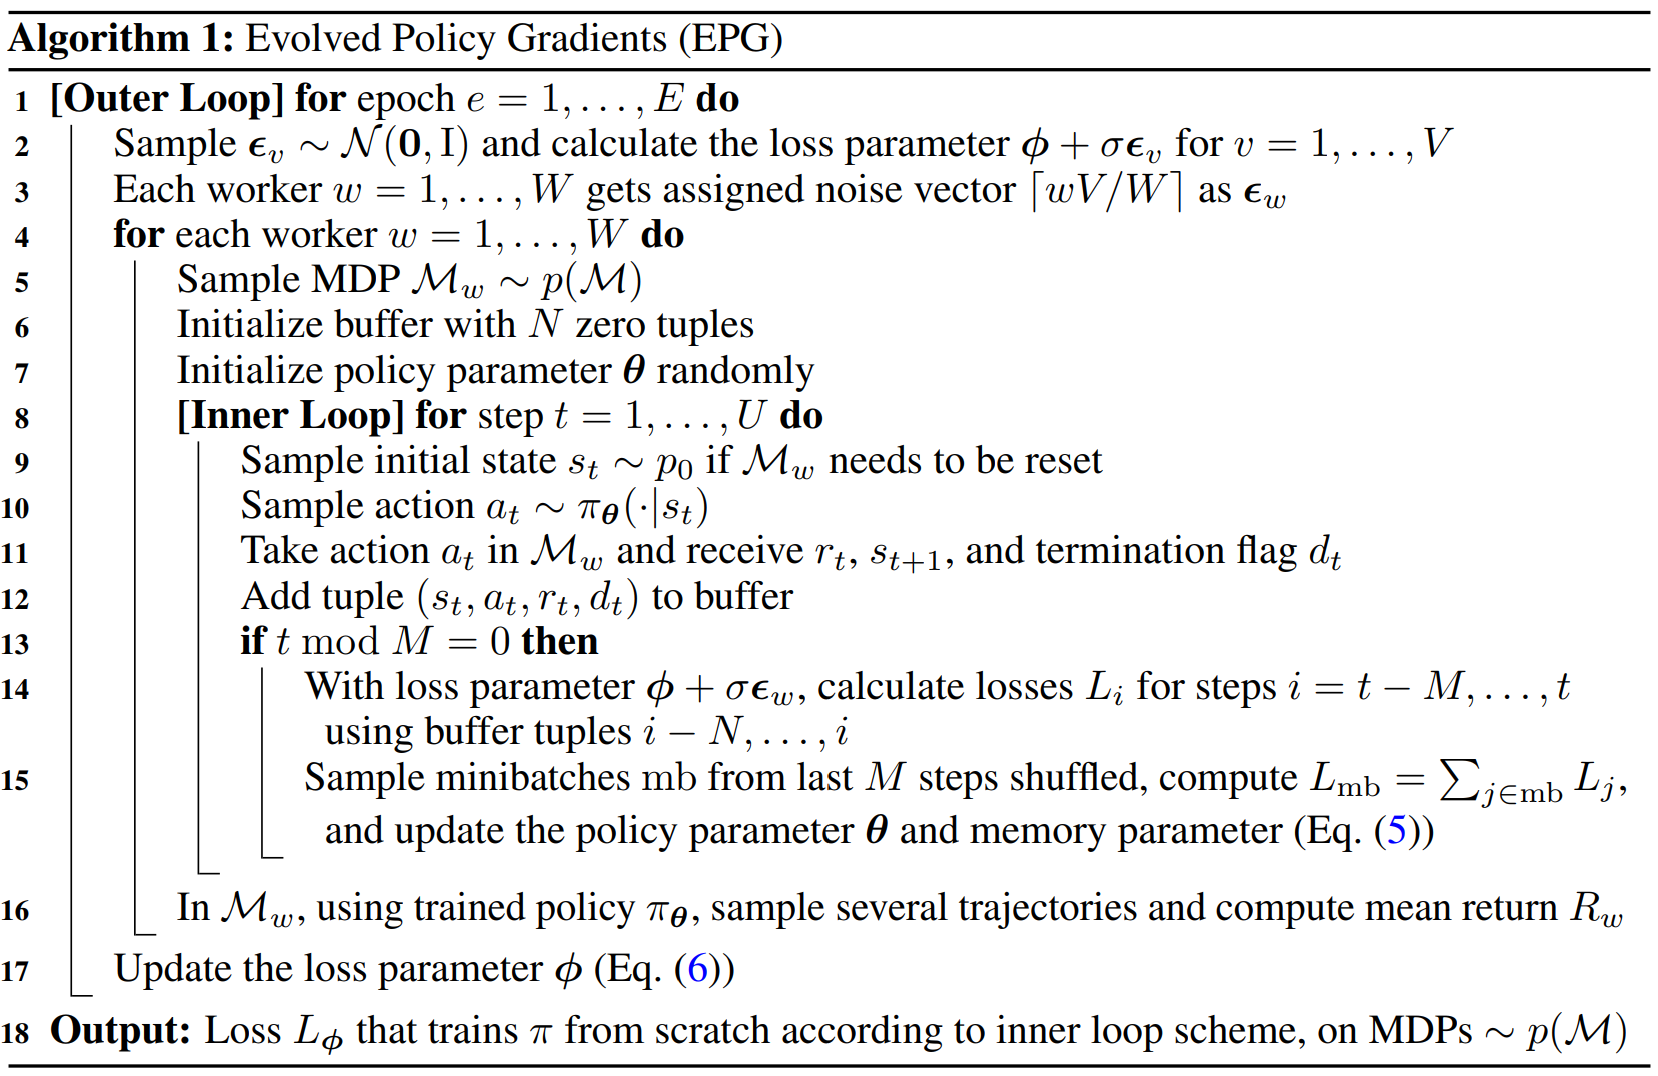
\includegraphics[scale=0.4]{epg.png}
	\centering
	\caption{EPG algorithm.}
	\label{epg}
\end{figure}

\par
The algorithm works as follows: Assumed that $\textit{W}$ workers are working in the inner loop. Then, at the beginning of each epoch in the outer loop, $\textit{V}$ multivariate normal vectors $\epsilon_v \in \mathcal{N}(0,I)$ of the same dimension as the loss function parameter $\phi$ are generated and assigned to $\textit{V}$ loss functions $L_\omega = L_{\phi+\delta\epsilon_v}$ respectively, with $\textit{v}$ being the $\textit{v}$-th generated perturbed parameters.

\par
Afterwards, the inner loop launches, each worker samples a random MDP from the task distribution $\mathcal{M}_\omega\thicksim p(\mathcal{M})$ and trains the policy $\pi_\theta$ along with the loss function $L_\omega$ given from the outer loop and updates the parameter $\theta$ as follows:

\[\theta\gets\theta - \delta_{in}\cdot\nabla_\theta L_\omega(\pi_\theta,\tau_{t-M,...,t})\]

\par
At the end of the inner-loop training, the return $R_\omega$ is returned by each worker and is aggregated in the outer loop. Then, the parameter $\phi$ of the loss function is updated according to the rule shown below:

\[\phi\gets\phi+\delta_{out}\cdot\frac{1}{V_\sigma}\sum_{v=1}^{V}F(\phi+\sigma\epsilon_v)\epsilon_v\]

where $F(\phi+\sigma\epsilon_v) = \frac{R_{(v-1)*W/V+1}+...+R_{v*W/V}}{W/V}$.

\par
The architecture of the loss function can be seen in the following figure:
\begin{figure}[H]
	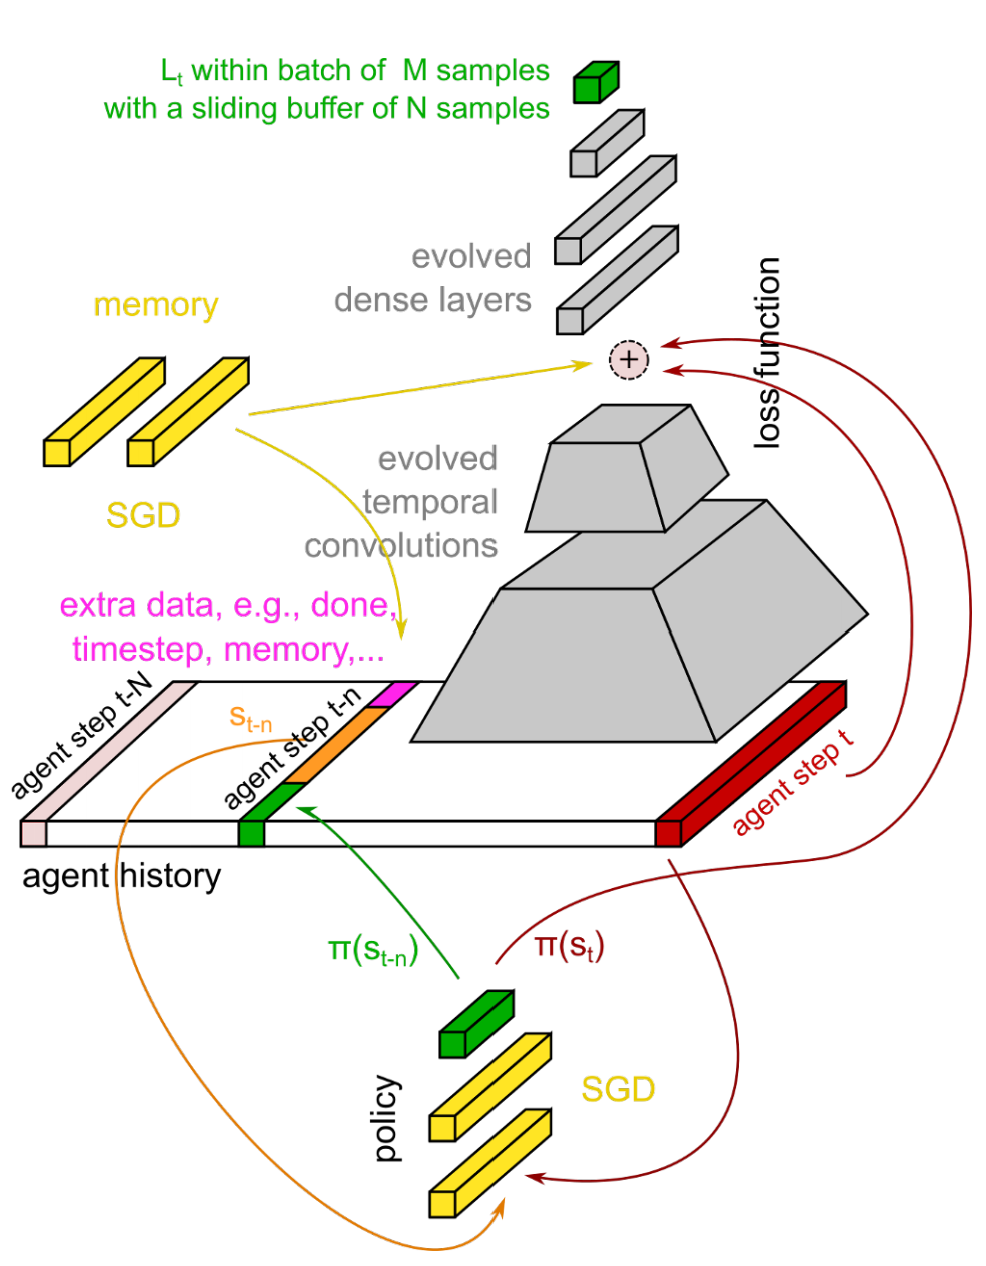
\includegraphics[scale=0.5]{loss-architecture.png}
	\centering
	\caption{Architecture of loss function $L_\phi$.}
	\label{loss-architecture}
\end{figure}

\par
As depicted in the diagram above, the architecture contains a memory unit, which is actually a single-layer neural network accepting constant input vector and is used to store the loss function value, as well as an experience buffer with limited storage, which stores the agent's \textit{N} most recent experience steps, in the form of a list of tuples $(s_t,a_t,r_t,d_t)$ at time step t, where \textit{$d_t$} is the trajectory termination flag.

\par
In addition, the architecture consists of temporal convolutional layers which generate a context vector $f_{context}$, and dense layers, which output the loss. The dense layer outputs the loss function \textit{$L_t$} at time step t by taking a batch of \textit{M} sequential samples $\{{s_i,a_i,d_i},mem,f_{context},\pi_\theta(\cdot|s_i)\}^t_{i=t-M}$. To generate the context vector, first, the data samples $\{{s_i,a_i,d_i},mem,\pi_\theta(\cdot|s_i)\}^t_{i=t-N}$ are stack together to form a matrix, second, this matrix is processed by the temporal convolutional layers which outputs the context vector $f_context$.

\par
This algorithm is evaluated under several randomized continuous control MuJoCo environments. For example, the following diagrams show results on RandomHopper, RandomWalker and RandomReacher.
\begin{figure}[H]
	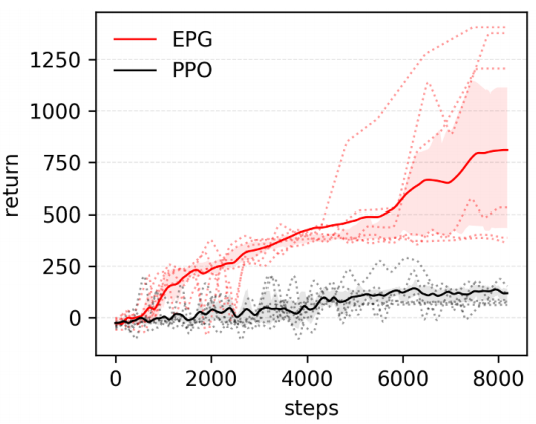
\includegraphics[scale=0.5]{hopper.png}
	\centering
	\caption{RandomHopper testtime training over 128 (policy updates) x64 (update frequency) = 8196 timesteps: PPO vs no-reward EPG.}
	\label{hopper}
\end{figure}
\begin{figure}[H]
	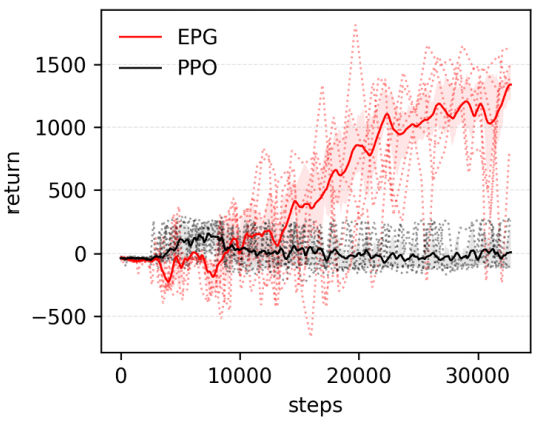
\includegraphics[scale=0.5]{walker.png}
	\centering
	\caption{RandomWalker testtime training over 256 (policy updates) x128 (update frequency) = 32768 timesteps: PPO vs no-reward EPG.}
	\label{walker}
\end{figure}
\begin{figure}[H]
	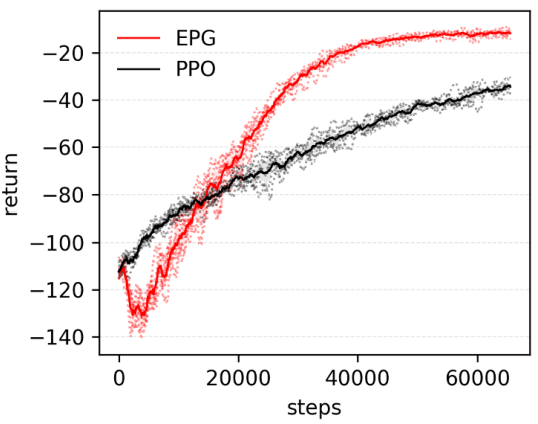
\includegraphics[scale=0.5]{reacher.png}
	\centering
	\caption{RandomReacher testtime training over 512 (policy updates) x128 (update frequency) = 65536 timesteps: PG vs no-reward EPG.}
	\label{reacher}
\end{figure}